\subsection{CU17 Modificar Refacción}
Cuando el administrador elige la opción de modificar un registro, se despliega esta pantalla donde el sistema muestra un formulario de actualización donde todos los campos están llenos con la información que está dentro de la base de datos. En la parte inferior de esta ventana tenemos dos botones:
\begin{itemize}
	\item \textbf{Modificar:} Al dar click en este botón, el sistema validará nuevamente todos los campos hayan sido modificados o no, validando si están llenos y su formato. 
	\item \textbf{Cancelar:} El sistema regresa a la pantalla anterior (figura \ref{fig:Pantalla Visualizar Refacciones Administrador - Vista de Escenarios}) sin modificar ningún dato. 
\end{itemize}
\begin{figure}[!h]
	\centering
	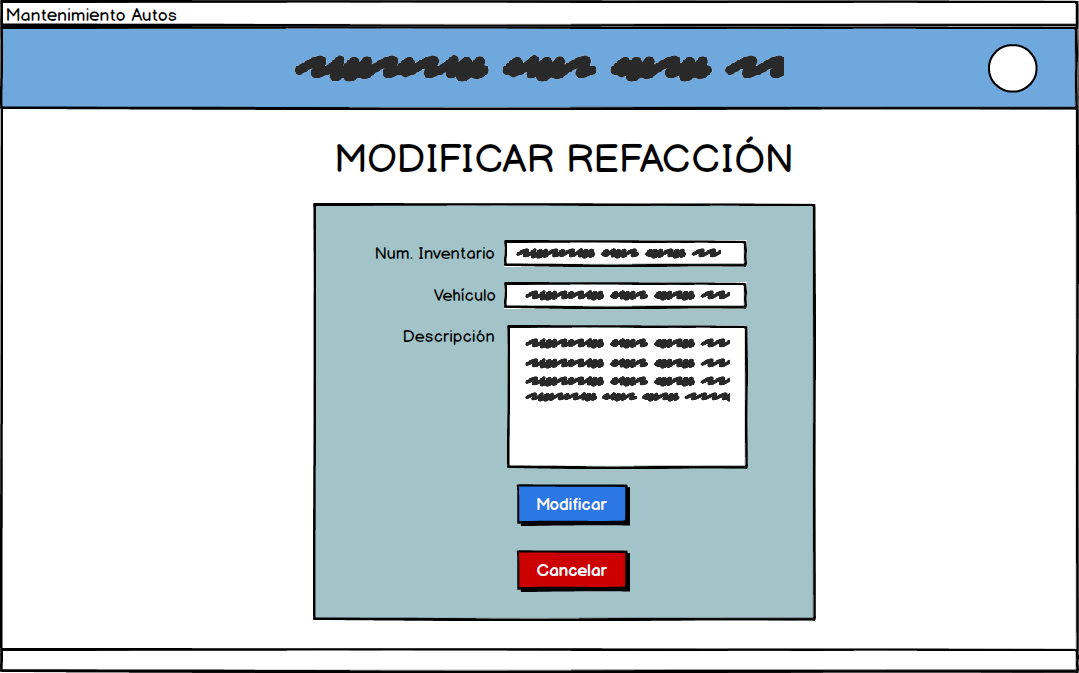
\includegraphics[width=0.8\textwidth]{./diseno/vescenarios/imagenes/modificarRefaccion}
	\caption{Pantalla Modificar Refacciones  - Vista de Escenarios}
	\label{fig:Pantalla Modificar Refacción - Vista de Escenarios}
\end{figure}
\begin{figure}[!h]
	\centering
	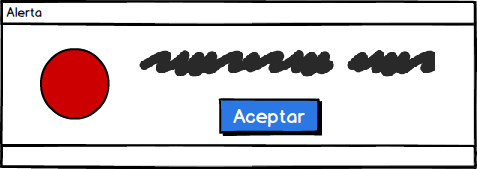
\includegraphics[width=0.3\textwidth]{./diseno/vescenarios/imagenes/alerta}
	\caption{Alerta Modificar Refacciones- Vista de Escenarios}
	\label{fig:Alerta Registro Refacciones - Vista de Escenarios}
\end{figure}
\clearpage